\RequirePackage{fix-cm}
%
%\documentclass{svjour3}                     % onecolumn (standard format)
%\documentclass[smallcondensed]{svjour3}     % onecolumn (ditto)
%\documentclass[smallextended]{svjour3}       % onecolumn (second format)
\documentclass[twocolumn]{svjour3}          % twocolumn
%
\smartqed  % flush right qed marks, e.g. at end of proof
%
\usepackage{graphicx}
%
\usepackage{mathptmx}      % use Times fonts if available on your TeX system
%
% insert here the call for the packages your document requires
\usepackage{latexsym}
\usepackage{url}
\usepackage{changepage}
\usepackage{amssymb,amsmath}
\usepackage[colorlinks,citecolor=blue,linkcolor=blue]{hyperref}
\usepackage{color}
\usepackage{mdwlist}
\usepackage{algorithm}
\usepackage{algorithmic}
\renewcommand{\algorithmicrequire}{ \textbf{Input:}} %Use Input in the format of Algorithm
\renewcommand{\algorithmicensure}{ \textbf{Output:}} %UseOutput in the format of Algorithm
%\spnewtheorem{definition}{Definition}{\bf}{\rm}
\spnewtheorem{hypothesis}{Hypothesis}{\bf}{\rm}

%
% please place your own definitions here and don't use \def but
% \newcommand{}{}
%
% Insert the name of "your journal" with
\journalname{Cognitive Computation}
%
\begin{document}

\title{Toward Tight Homophily: Modeling Subjectivity of Social Media User for Behavior Analysis%\thanks{Grants or other notes
%about the article that should go on the front page should be
%placed here. General acknowledgments should be placed at the end of the article.}
}
%\subtitle{Do you have a subtitle?\\ If so, write it here}

%\titlerunning{Short form of title}        % if too long for running head

\author{Songxian Xie         \and
		Jintao Tang           \and
        Ting Wang %etc.
}

%\authorrunning{Short form of author list} % if too long for running head

\institute{Songxian Xie \at
              school of computer, National University of Defense Technology \\
              Tel.: +86-0731-84574627\\
%              Fax: +123-45-678910\\
              \email{xsongx@nudt.edu.cn}            \\
%             \emph{Present address:} of F. Author  %  if needed
%           \and
           Jintao Tang \at
              Jttang@nudt.edu.cn \\
           Ting Wang \at
              tingwang@nudt.edu.cn
}

\date{Received: date / Accepted: date}
% The correct dates will be entered by the editor


\maketitle

\begin{abstract}
Retweeting is the core mechanism of information diffusion on Twitter, and many factors have been proved to influence retweeting behavior, however few studies have investigated the subjective motivation of a user to retweet a message. 
Subjective nature of human is the underlying reason of diverse social behaviors including information diffusion, and subjective resonance triggered by topics and opinions similarity between tweets and users will elicit retweeting.
In this paper, in the light of psychological theory, we assume that a tweet is more likely to be retweeted by a user because of similar subjectivity, and propose a subjectivity model  to combine both the topics and opinions to model subjectivity. 
With state-of-the-art topic model and sentiment analysis techniques, we establish subjectivity model  by finding topics and determining opinions towards these topics from user-generated content simultaneously.
We evaluate our model in the retweeting analysis problem to verify its impact on retweeting and effectiveness in the retweeting prediction performance. 
Specifically, we demonstrate that subjective similarity is the most distinguishable feature with largest difference between retweeted and unretweeted users;
subjectivity model  outperforms other models in rewteeting prediction; 
and features derived from subjectivity model  give the most significant improvement over a off-the-shelf predicting model in a classification framework.
\keywords{Twitter \and subjectivity \and retweeting behavior \and LDA \and sentiment analysis}
% \PACS{PACS code1 \and PACS code2 \and more}
% \subclass{MSC code1 \and MSC code2 \and more}
\end{abstract}

\section{Introduction}
\label{intro}

They provide access to a very vast source of information on an unprecedented scale. \textit{De facto}, an online social network (OSN) can be described as a user-generated content system that permits its users to communicate and share information.
Messages are the main information vehicle in such services. Users publish messages to share or for-ward various kinds of information, such as product recommendations, political opinions, ideas, etc.
More data about social behavior is now available than ever
before. These data, much of which come from social media sites such as Twitter, contain traces of individual activity and social interactions. On Twitter, interactions include users posting short text messages, called tweets, and following other users to receive their posts. Users may also respond to posts shared by others, for example, by retweeting them to their own followers. These abundant data offer new opportunities for learning models of user behavior and interests, identifying communities of like-minded users, and inferring the topics of conversations between them. The models can, in turn, be used to understand how popular opinion is changing, predict future activity, and identify timely and interesting information.
Researchers have developed a variety of probabilistic meth-
ods to learn user models from social data \cite{chua2013generative,kang2013lda,wang2011collaborative,purushotham2012collaborative}.
Such models usually include a user’s interest in some topic as a hidden parameter, which is estimated from her response to messages on that topic. The more a user responds, for example, by retweeting a message on the topic, the more she is interested in it. These models, however, fail to account for details of user behavior that affect response, such as how often the user visits Twitter, how many messages she receives, and how many of these she inspects. Without considering these variables, it is difficult to explain behavior. Does a lack of response mean that a user is not interested in the topic, or
that that she simply did not see the message? These probabilistic models also need large amounts of data to learn accurate models, which may not be obtainable for all users.

we compartmentalize, or group, users by their activity, interest in the topic and number of friends. This means that the model treats users with the same number of friends and same activity level as indistinguishable from each other when computing transitions between states, thereby ignoring additional individual differences. This simplification makes stochastic models tractable by reducing the number of parameters necessary to describe the population.

Over the past forty years, social network theorists have
been interested in studying the factors at play behind forma- tion of ties between individuals. A tie, typically reflecting a psychological or sociological relationship, defines the topo- logical characteristics of a network at large. It is responsible for affecting the spatio-temporal dynamics encompassing a number of social phenomena in networks—including how information propagates from one individual to another, or how communities emerge and evolve around shared relationships.

In particular, extracting user’s interests with the content of document simultaneously has received considerable attention in recent years. This has led to the proposal of various topic models that can infer latent topics with author’s interests automatically, where each topic is a latent variable that has a probability distribution over words. These topic models introduce author’s interests as topic distributions according to their document contents. These proposed topic models aim at using topics or sets of topics to represent author’s interests and provide useful description for the generative process of various data, which could be applied in different aspects such as social network analysis, expertise recommendation  and collaborative filtering , etc. \cite{zhao2012user}
However, most topic models combined with author’s information have not considered author’s sentiment with his interested topics.
However, these works could not study well on user’s interest level but just in documents level.It is essential to identify user’s sentiment to his interests. According to the previous probability generative model, topics or user’s interests are extracted only with the probability of co-occurrence, which means if a user talks about one topic frequently, the models will consider that the user is interested in it but do not care the sentiment trend on the topic. Users who talk much about a topic could have different opinions about it. It is better to distinguish these users instead of viewing them in the same community. For example some people talk a lot about the topic they like, while even if others dislike it, they could also discuss a lot about it in negative aspects. In conventional methods, these users will be clustered in the same community, but it is obvious that people with different opinions should be separated.One thing should be noted that our model considers sentiment and topic simultaneously, by which it makes that not all extracted topics have both positive and negative sentiment trends.

\section{Related Works}
Recently, the researching works about topic model have focused more on two aspects, i.e., topic models combined with author’s information and topic models combined with sentiment information. Topic model is a stream of new research in machine learning and natural language models for clustering words in order to find the underlying topics. Latent Dirichlet Allocation (LDA) \cite{blei2003latent} can robustly discover multinomial word distributions of these topics. When merging author’s information in topic model, some extended works based on LDA have been proposed, Author-Topic model \cite{steyvers2004probabilistic} learns topics conditioned on the mixture of authors that composed a document which each author has a distribution over topics, Author-Persona Topic model \cite{mimno2007expertise} allows each author’s documents to be divided into several clusters in order to find personas of the author by the topic distribution over these documents clusters. Compared with these works that represent author’s interests or personas by topic distribution, Author Interest Topic model (AIT) \cite{kawamae2010author} considers adding a document class layer between the author layer and the topic layers which represents the author’s interests as a mixture of document classes. Latent Interest Topic model (LIT) \cite{kawamae2010latent} is extended from AIT by adding an author class layer to model the relations between different authors, while Role-Author-Recipient model \cite{mccallum2005topic} considers the roles of users by assigning a role-layer to the
pair of author and recipient. Moreover, researching works have tried to utilize the semantic analysis of topic model with social graph to detect communities. In \cite{zhou2006probabilistic}, the authors proposed the CUT (Community-User-Topic) model which discovered communities using semantic content of the social graph. One of the first attempts to combine link based community discovery methods with content based method is the Community-Author- Recipient Topic (CART) model \cite{pathak2008social}. However, since CART, there have been few advanced attempts on combining link and content analysis to detect communities more effectively. The Topic-Link LDA model \cite{liu2009topic} and Rational Topic Models \cite{chang2009relational} draw latent topical and community distributions for each node in documents networks. Then they generate links between documents based on topical similarity and community membership similarities of their authors. All these works have shown the availability of topic models to do Social Network Analysis but they all ignore the sentiment information among the topics. When combined sentiment detection with topic models, this probability generative model works also show a strong suitability. Several unified models of topics and sentiment have been proposed, and they extend basic topic model works to explain the sentiment trends with topic from documents such as reviews or comments \cite{mei2007topic,lin2009joint,jo2011aspect}. Topic Sentiment Mixture (TSM) model \cite{mei2007topic} represents the sentiment as a language model separated from topics, which means TSM considers the topic and sentiment separately, the word samples from either topics or sentiments. Multi-Aspect Sentiment (MAS) model \cite{jo2011aspect} aims at modeling topics to the predefined aspects that are explicitly rated by users in reviews, from which the sentiment is modeled on the aspect level according to the sentiment distribution from a weighted combination from extracted topics and words. Joint Sentiment/Topic (JST) model \cite{lin2009joint} presents a novel way to detect the sentiment of document with topic extraction and its sampling process considers that the topics are associated with sentiment and document, which can model the topic and sentiment simultaneously. JST takes much similar way as our work but it only detects the sentiment on document level. Moreover, to limit the meaning of extracted topics, extra labels or constraints are incorporated into topic model frameworks. Labeled-LDA \cite{ramage2009labeled} is a supervised topic model for credit attribution in multi-labeled corpora, which constrains each topic from particular labels by assigning different prior probabilities from multi-labels in the corpora. From this definition, the topics extracted by Labeled-LDA are more meaningful and distinguishable towards labels. Our proposed model learns the idea from Labeled-LDA to distinguish the sentiment labels of topics. However, our model needs only a general sentiment paradigm word list but Labeled-LDA needs to provide labels to each document in the corpora.

To the best of our knowledge, such an integration problem has not been studied in the existing work.\cite{lu2008opinion}

Furthermore, a lot of current opinion mining work focuses on mining review data and solving classification problems. As we go beyond product reviews, only knowing sentiment orientations such as positive, negative and neutral is not enough in many cases. This is especially true in the domain of politics where the wording is often sensitive. For exam- ple, with respect to healthcare reform in U.S., a Republican might often say “we want responsible healthcare reform based on private insurance”1, while a Democrat might often say “we want universal healthcare reform with a public government-run health insurance agency”. Both statements can be viewed as positive on healthcare reform in general, but the opinion words“responsible”and“private”vs“universal” and “public” reflect their huge difference on the issue.Therefore, in COM, the opinions of interest are represented by opinion words which are directly returned to users.\cite{fang2012mining}

As the reason of that, Twitter has three features: convenience,immediacy and propagating.\cite{ikegami2013topic}
Twitter facilitates real-time propaga- tion of information to a large group of users. This makes it an ideal environment for the dissemination of breaking-news directly from the news source and/or geographical location of events.\cite{castillo2011information}

Review data is relatively easier to work with since sentences in reviews are more grammatically correct compared to tweets. Tweets on the other hand are short, informal, colloquial, and can contain slangs and abbreviations. Thus, many of the existing natural language processing tools such as Part-of-Speech (POS) tagger, tokenizer, and dependency parser fail to work well because they are typically trained on newswire data.Instead, current Twitter sentiment analysis approaches \cite{barbosa2010robust,davidov2010enhanced,go2009twitter,read2005using,saif2012alleviating} adopt a machine learning approach similar to text classification.Training data are often obtained by using noisy labels (also known as distant supervision). This allows us to classify the tweets without manual supervision. Go et al. \cite{go2009twitter} and Read \cite{read2005using} exploit emoticons such as “:-)” and “:-(“ to label the tweets positive and negative respectively. They then treat the problem as a text classification task and use machine learning techniques such as Naïve Bayes (NB), Maximum Entropy (MaxEnt), and Support Vector Machines (SVM) to train a classifier. Barbosa and Feng \cite{barbosa2010robust} on the other hand, construct their training data from a few different Twitter sentiment analysis websites.\cite{lek2013aspect}

For example, there are several words that are written informally like “nooooooooooooo”, “loveeeeeeeeeee”,“sundayssss”, “saddddddd”,“xxplosive”, “foooooooood”,”okaaay” and so on. A sentiment is often represented in subtle or complex ways in a text. An online user can use a diverse range of other techniques to express his or her emotions. Apart from that, s/he may mix objective and subjective information about a certain topic. On top of that, data gathered from the World Wide Web often contain a lot of noise. Indeed, the task of automatic sentiment recognition in online text becomes more difficult for all the aforementioned reasons.

For example, Tan et. al. \cite{tan2011user} utilized the social connection to improve the sentiment classification performance based on the intuition that connected users are more likely to share similar opinions towards the same entity. 

in many applications, the polarity should be on the user instead of a single document. In fact, the quality of a single document (e.g., a product review) may vary largely, even for the same user. \cite{tang2013sentiment}


Tan et al. \cite{tan2011user} study the problem of user-level sentiment analysis using social networks. we employ the assumption that the influence between the nodes only occurs within distance of 1. Thus a user’s sentiment is only influenced by himself and his followees.We work within a semi-supervised, user-level framework. The
reason we adopt a semi-supervised approach is that the acquisition of a large quantity of relevant sentiment-labeled data can be a time- consuming and error-prone process, as discussed later in this pa- per. We focus on user-level rather than tweet-level (corresponding to document- or sentence-level) sentiment because the end goal for many users of opinion-mining technologies is to find out what peo- ple think; determining the sentiment expressed in individual texts is usually a subtask of or proxy for that ultimate objective. Addition- ally, it is plausible that there are cases where some of a user’s tweets are genuinely ambiguous (perhaps because they are very short), but his/her overall opinion can be determined by looking at his/her col- lection of tweets and who he/she is connected to. 
when a user forms a link in a net- work such as Twitter, they do so to create a connection. If this connection corresponds to a personal relationship, then the prin- ciple of homophily \cite{lazarsfeld_friendship_1954} — the idea that similarity and connection tend to co-occur, or “birds of a feather flock together” \cite{mcpherson2001birds}—sug- gests that users that are “connected” by a mutual personal relation- ship may tend to hold similar opinions; indeed, one study found some evidence of homophily for both positive and negative senti- ment among MySpace Friends \cite{thelwall2010emotion}. Alternatively, the connection a user creates may correspond to approval (e.g., of a famous figure) or a desire to pay attention (e.g., to a news source), rather than nec- essarily a personal relationship; but such connections are still also suggestive of the possibility of a shared opinion.
First, we empirically confirm that the probability that two users share the same opinion is indeed correlated with whether they are connected in the social network.
since the Twitter
interface makes the tweets of t-followee vj visible to t-follower vi (and similarly for @-mentions), so we have some reason to believe that vi is aware of vj’s opinions.
In this section, we frame the problem in the context of Twitter to keep things concrete, although adaptation of this framework to other social-network settings is straightforward.\cite{tan2011user}

Emotion is now recognised as an important aspect of many areas of our lives. Aside from the obvious relevance of feelings like happiness and sadness to personal well–being, appropriate perception and communication of emotion is important for maintaining human relationships and friendships and not just intimate relationships. Particularly for women, friends are also a source of emotional support, one that can help individuals to cope in difficult times.\cite{stoppard1993gender}, it is important to understand as much as possible about the properties of online emotion expression and support in friendship, so that appropriate actions can be taken if the important social institution of friendship is under threat or, conversely, if new opportunities are evident.

There are many socially recognised types of emotion, such as happiness, fear,sadness and anger, but one common way of analysing emotion is in terms of the two dimensions of valence and arousal \cite{cornelius1996science}. Valence is the type of emotion felt: the extent to which it is positive or negative. Arousal is the general perceived level of activation or energy and it is often associated
with the strength of an emotion. Hence it is reasonable to simplify a discussion of emotions in friendship to just valence/polarity and strength. Note, however, that it is possible to simultaneously experience or express positive and negative emotions \cite{fox2008emotion}: to have mixed feelings about an event.
An emotion categorisation program (Thelwall, et al., submitted) was used to assign a positive and a negative emotion to each comment on a scale of one (no emotion) to five (very strong emotion). The classification was based upon a predefined list of about 500 emotion–bearing words (e.g., hate = negative 4), emoticons and emphatic devices including words (e.g., very), punctuation (e.g., !!!!) and repeated letter emphatic spelling (e.g., soooo).\cite{thelwall2010emotion}

The central issue addressed in this paper is homophily, the tendency for friendships and many other interpersonal relationships to occur between similar people. Based upon a survey of predominantly US research, it seems that gender, sexuality, religion, race and age similarity are all important predictors of friendship\cite{mcpherson2001birds}.\cite{thelwall2009homophily}

micro-blogs differ by (1) placing a strict limit on length, resulting radically in new forms of emotional expression, and (2) encouraging users to express their daily thoughts in real-time, often resulting in far more emotion statements than might normally occur. Micro-blogging services such as Twitter provide researchers with a wealth of information on how individu- als communicate with their social network. Unlike more formalmethods of communication,micro-blog posts (here- after, “tweets”) frequently reflect the author’s opinions and emotional states. For instance, Table 1 shows several re- cent tweets reflecting on the latest FIFA World Cup. Fur- thermore, since tweets are restricted to 140 characters, and since they are oftenwritten onmobile devices, they express emotions less formally than other publishing platforms.Such a systemwould be useful in understanding users’ feelings towards particular products, services, or topics (e.g., companies could deter- mine the distribution of emotions toward their latest product).\cite{roberts2012empatweet}

A prerequisite of all such research is an effective method for measuring the sentiment of a post or tweet. Due to the extremely informal nature of the medium, and the length restriction1, the lan- guage and jargon which is used in Twitter varies sig- nificantly from that of commonly studied text cor- pora. In addition, Twitter is a quickly evolving domain, and new terms are constantly being introduced.
In purely text-based domains, such as Twitter, styling is not always available, and is replaced by capitalization or other conventions (e.g., enclosing the word in as- terisks). Additionally, the informal nature of the do- main leads to an orthographic style which is much closer to the spoken form than in other, more formal, domains.the commonly observed phenomenon of lengthening words by repeating letters is a substitute for prosodic em- phasis (increased duration or change of pitch). As such, it can be used as an indicator of important words and, in particular, ones that bear strong in- dication of sentiment.Phenomena include mis- spellings, abbreviations (e.g. “gr8” - “great”), emphatic uppercasing (“WHAT THE HELLWAS THAT????”), emphatic lengthening (“The concert was greeeeeeeeeaat!!!”) and the use of slang and neologisms. This leads to much more sparsity in the input and is a special chal- lenge for the use of lexical resources. Brody and Diakopoulos \cite{brody2011col} find emphatic lengthening to occur in every 6th tweet of their dataset and provide a detailed analysis.\cite{brody2011col}

Beside being an interesting research problem, sentiment analysis can be di- rectly applied by persons interested in a large amount of opinions towards a certain topic. 
With the rise of social media, the number of opinions on the web has multiplied, as platforms like Facebook and Twitter make it very easy for ev- eryone to share their thoughts on literally anything. This calls for sentiment analysis systems that can process large amounts of data and are able to han- dle the special challenges of the text genre of so-called microblogs. Because of the interest in utilizing this freely available information by research and industry, sentiment analysis of microblogs has become a popular research topic during the last years. Besides the challenges traditional sentiment analysis systems face, such as ambiguity, handling of negation, detection of sarcasm and opinion spam, sentiment analysis of microblogs have to handle the following additional difficulties:Text Length: Microblog posts are usually very short. While this can be an advantage, because authors tend to get straight to the point they want to make, it poses the challenge that the expressed opinion might be dependent on one word only. The word might not be available in the used lexical resource or might not have occurred in the training data, which can lead to the loss of the opinion. A discussion of the phenomenon can be found in Bermingham and Smeaton (2010).
Spelling variation: Due to spontaneity, the informal context and length restrictions the spelling in microblog posts tends to have much greater variability than in other text genres. Phenomena include mis- spellings, abbreviations (e.g. “gr8” - “great”), emphatic uppercasing (“WHAT THE HELLWAS THAT????”), emphatic lengthening (“The concert was greeeeeeeeeaat!!!”) and the use of slang and neologisms. This leads to much more sparsity in the input and is a special chal- lenge for the use of lexical resources. Brody and Diakopoulos (2011) find emphatic lengthening to occur in every 6th tweet of their dataset and provide a detailed analysis.
•Special tokens: Tokens uncommon in other text genres, such as URLs and emoticons, can lead to difficulties when trying to use natural language processing tools, such as part-of-speech taggers and syntactical parsers. The latter are often trained on newspaper texts, which are considerably different to microblog posts.
• Topic variation: The topics discussed on Twitter are not constrained in any way and the variety is therefore very large. This can cause problems for sentiment analysis, e.g. when words express different sentiment in different contexts.
Amount of data: While the texts as such are often short, the amount of texts can be overwhelmingly large. In 2012 the popular microblog-
ging service Twitter announced1 12,233 posts per second about the American football Super Bowl towards the end of the game.
• Language style: Due to Twitter’s large userbase the variety in writing style is very large. This might range from formal newspaper-like text to
very informal slang including profanity. Furthermore, the vocabulary used can change rapidly. All this can lead to problems for annotated training data and lexical resources.
• Multilingual content: While online newspapers and blogs tend to be written in one language, users of microblogging platforms use a wide variety of languages, sometimes even in the same message or sentence. With the shortness of the posts language detection becomes increas- ingly difficult.
These difficulties do not apply to sentiment analysis exclusively, but are also of concern for other natural language processing tools, such as part-of- speech taggers, parsers and the like.



There’re two important factors that should be taken into consider- ations. One, opinions and topics are closely related.The online discussions around some entity, or object, often cover a mixture of features/topics related to that entity with different preferentials. Different opinions may be expressed by users towards different topics, where users may like some aspects of an entity but dislike other aspects. Two, users’ opinions are subject to social influence. The rise of social media puts the sentiment analysis in the context of social network. Users not only express their individual opinions, but also exchange opinions with others. In the context of opinion mining, social influence refers to the phenomenon that one is inclined to agree (positive influence) or disagree (negative influence) with his/her neighbors’ opinions with different degrees, depending on the influence strengths.\cite{li2012mining}

As a real-time conversational platform Twitter presents a number of interest-ing user modeling and profiling opportunities and challenges. Twitter users are connected in relatively dense social networks of followers and friends and these networks can contain communities of users with shared interests. In addition, the conversations that take place within these networks, and the information
that is shared through these conversations, has the potential to provide a rich source of user preference and interest data, notwithstanding the 140-character limit that is placed on user posts.In recent work \cite{hannon2010recommending}, the text content of Twitter messages from a user and their followers/friends was used as the basis for text-based profiles as part of a recommendation system to suggest new users to follow. In this work, recommended users were suggested on the basis of term overlaps between the target user’s profile and the profiles of other users. Other researchers have ex- plored Twitter information to model users as the basis for news recommendation \cite{Abel:2011AUM,phelan2011terms} based on term overlap between news story content and user tweets.
One of the challenges with using tweet content as the basis for profiling is that it can lead to very large but noisy user profile \cite{liao2012mining}.We propose that this regioned, multi-faceted approach to profiling Twitter users provides an effective way to model the interests and preferences of users in a way that facilitates a better understanding of core and peripheral interests and also provides for a powerful framework for exploring a space of interests within Twitter’s social graph.

Twitter is well-known for its freedom of publishing short message (i.e. tweet), and viral spreading of information across complex social networks.
%Since launched in March 2006, the service rapidly has gained worldwide popularity, with over 500 million registered users at the end of year 2012, who generated over 340 million tweets per day\footnote{\url{http://en.wikipedia.org/wiki/Twitter}}.
In addition to large amounts of User-Generated Content (UGC), Twitter provides its social network functions for connection, communication and information diffusion by allowing users to message one another directly and follow one another publicly. 
The complex networks and large content volume of Twitter provide researchers with insights into people’s social behaviors on a scale that has never been possible \cite{DBLP:conf/hicss/StieglitzD12}.

Information diffusion is a challenging problem which might be investigated on Twitter, because retweeting convention and complex networks of Twitter have provided an unprecedented mechanism for the spread of information despite the restricted length of tweets \cite{Jenders:2013APV}. 
Actually almost 25\% of the tweets published by users are retweeted from others \cite{conf/cikm/YangGCTLZS10}. 
Therefore, it is important to understand how retweeting behavior works which can help study information diffusion on Twitter. 

Although several works have concentrated on analyzing retweeting habits and influencing factors \cite{Boyd2010,Kwak:2010TSN,Suh2010}, most of them are generic, not user-oriented.
From the point of a user, retweeting is a process that includes reading the tweet, estimating the content and deciding to share, and the crucial part of the process is to estimate whether a tweet contains information interesting to the user who might find it worthy to be shared.
Therefore in this study we focus specifically on analyzing the retweeting behavior from the user modelling perspective.

Previous studies on retweeting analysis have shown that an enriched user model gives coherent and consistent explanation for retweeting motivation\cite{Abel:2011AUM,conf/icwsm/MacskassyM11,conf/wsdm/FengW13}. 
Specifically, researchers have tried to model users from four types of information:
profile features ("\textbf{Who you are}"), tweeting behavior ("\textbf{How you tweet}"), linguistic content ("\textbf{What you tweet}") and social network ("\textbf{Who you tweet}") \cite{Pennacchiotti:icwsm11}. 
Despite demographic profile, tweeting habits and network structure might determine the source and scope of information users could be exposed to, topics of interest encapsulated in rich linguistic content have been proved consistently dependable for retweeting behavior explanation. 
For example, Petrovic \emph{et al.}~\cite{Osborne_Lavrenko_2011} and Hong \emph{et al.}~\cite{ericmedvet:hong2011} found whether a tweet will be propagated largely depends on its identification with the interests of users. 
However, beyond merely publishing news and events, Twitter has become a platform where different opinions are presented and exchanged by allowing users publish subjective messages on topics they are interested in. 
Existing researches demonstrated that UGC with rich sentimental information can trigger more attention, feedback or participation \cite{DBLP:conf/hicss/StieglitzD12}, and tweets with high emotional diversity have a better chance of being retweeted \cite{conf/icwsm/PfitznerGS12}.
Most studies have tried to find whether and how sentiment of a tweet will influence its spreading, but none of them realize that although users receive thousands of tweets on different topics every day, whether a tweet will be retweeted will depend on the subjective choice of users. 

Subjective initiative nature of human determines that his behavior pattern is subjectivity driven.
Psychologist have identified subjectivity as the underlying factor that influences taking what behaviors to process incoming stimul \cite{Moore2008}.
According to theory of Biased Assimilation, people are prone to choose and diffuse information according to their own biased subjectivity \cite{Hyman2000,sunstein2009rumors}. 
In this study we explore the UGC of Twitter to model the subjectivity of users, and investigate whether the subjectivity model could benefit the retweeting behavior analysis. 
Intuitively, subjectivity can be represented as topics and opinions articulated in the information generated by users on Twitter.
We use the state-of-the-art topic model to find the topics users are talking about, and sentiment analysis techniques to determine user's opinions towards these topics from UGC simultaneously. 
We evaluate our model on the retweeting analysis problem to verify its impact on retweeting behavior.

Modelling subjectivity on Twitter is a challenging task because of the sparsity of textual information and the dynamic of topics and opinions.
However, we are interested in understanding retweeting behavior at a local level rather than at a global level, since most of time retweeting pertains to a local network consisting of the tweet publisher and followers, and the relatively tiny size and topic homophily of local network lower the impact of sparsity.
Given the biased nature of subjectivity, while new information may arise and old information may change their meaning, biased subjectivity is likely to be more consistent and less prone to external perturbations, therefore subjectivity model  of a user is less likely to be influenced by changes of topics and opinions on Twitter.
 
Our work aims to define and establish the subjectivity model  and identify the role of subjectivity in the processes of information diffusion on Twitter. Our contributions can be summarized as follows:
\begin{itemize}
\item In the light of psychological theory, we firstly put forward formal definition of subjectivity model  for users and tweets which model both the topics and opinions simultaneously.
\item Based on the state-of-the-art topic model and sentiment analysis techniques, we build subjectivity model from UGC on Twitter and apply it to the retweeting behavior analysis problem. 
\item We systematically evaluate the effectiveness of the subjectivity model. It is demonstrated that our model outperforms other UGC-based models in rewteeting prediction and gives the most significant improvement over a off-the-shelf predicting model. 
\end{itemize}
The rest of the paper is organized as follows: section 2 gives the related work to our research, the proposed subjectivity model  is defined and specified in section 3, the qualitative and quantitative evaluation is described in section 4, and Section 5 summarizes the paper and points out future work.

\section{Related Work}
\label{relatedwork}

\paragraph{Retweeting Analysis.}
A lot of works have analyzed the characteristics of retweeting, examining factors that lead to increased retweetability and designing models to estimate the probability of being retweeted. 
As for factors influencing retweetability, Suh \emph{et al.}~\cite{Suh2010} found that tweets with URLs and hashtags were more likely to be retweeted. 
Macskassy and Michelson~\cite{conf/icwsm/MacskassyM11} found that models derived from tweet content could explain most of retweeting behaviors.
Comarela \emph{et al.}~\cite{Comarela:2012UFA} found previous response to the tweeter, the tweeters’ sending rate, the freshness of information, the length of tweet could affect followers’ response to retweet. 
Starbird and Palen~\cite{Starbird:2012RRI} found that tweets with topical keywords were more likely to be retweeted. 
There are also many works extending the analysis to build retweeting prediction model. 
Osborne and Lavrenko~\cite{Osborne_Lavrenko_2011} introduced features such as novelty of a tweet and the number of times the author is listed to train a model with a passive aggressive algorithm, and found that tweet features added a substantial boost to the performance. 
Jenders \emph{et al.}~\cite{Jenders:2013APV} analyzed the "obvious" and "latent" features from structural, content-based, and sentimental aspects and found a combination of features covering all aspects was the key to high prediction quality.
Naveed \emph{et al.}~\cite{Naveed:2011SMC,2011:NaveedGKC} introduced interestingness based on such features as sentiments and topics to predict the probability of retweeting for an individual tweet.
Feng and Wang~\cite{conf/wsdm/FengW13} proposed a feature-aware factorization model to rerank the tweets according to their probability of being retweeted.
Pfitzner \emph{et al.}~\cite{conf/icwsm/PfitznerGS12} proposed a new measure called emotional divergence and showed that high emotional diverse tweets have higher chances of being retweeted.

All papers introduced above tried to answer the question of ``Whether and why a tweet will be retweeted by anyone''. 
But they are weak to capture ``Whether a tweet is retweetable from a user-centric perspective considering the interests and opinions ''. 
In this paper, we will try to answer this question by building a subjectivity model  which can capture both the interests and opinions of users.

\paragraph{User Modelling.}
With the popularity of social media, researchers have begun to pay close attention to model users on the massive amount of UGC. These studies provide researchers with insights into user online behaviors. 
Hannon \emph{et al.}~\cite{Hannon:2010} proposed that Twitter users can be modeled by tweets content and the relation of Twitter social network.
Macskassy and Michelson~\cite{conf/icwsm/MacskassyM11} discovered user's interests by leveraging Wikipedia as external knowledge to determine a common set of high-level categories that covers entities in UGC. 
Ramage \emph{et al.}~\cite{RamageEtAl:10} made use of topic models to analyze tweets at the level of individual users with 4S dimensions, showing improved performance on tasks such as post filtering and user recommendation. 
Xu \emph{et al.}~\cite{Xu:2012MUP} proposed a mixture model which incorporated three important factors, namely breaking news, friends' timeline and user interest, to explain user posting behavior.
Pennacchiotti and Popescu~\cite{Pennacchiotti:icwsm11} proposed a comprehensive method to model users for user classification, and confirmed the value of in-depth features by exploiting the UGC, which reflect a deeper understanding of the Twitter user and the user network structure.

Few of work have identified the correlation between the opinions of users and their behaviors, motivated by the observation, we put forward subjectivity model to combine both interests and opinions to model a user.

\paragraph{Sentiment Analysis.}
Sentiment analysis is a popular research area and previous researches have mainly focused on reviews or news comments. 
Recently, researchers began to pay more and more attention to social media such as Twitter.  
Hu \emph{et al.}~\cite{Hu:2013www} interpreted emotional signals available in tweets for unsupervised sentiment analysis by providing a unified way to model two main categories of emotional signals: emotion indication and emotion correlation. 
Jiang \emph{et al.}~\cite{Jiang:2011TTS} focused on target-dependent Twitter sentiment classification, and proposed a method to improve performance by taking target-dependent features and related tweets into consideration. 
Asiaee T. \emph{et al.}~\cite{AsiaeeT:2012} presented a cascaded classifier framework for per-tweet sentiment analysis by extracting tweets about a desired target subject, separating tweets with sentiment, and setting apart positive from negative tweets.
Hu emph{et al.}~\cite{Hu:2013ESR} extracted sentiment relations between tweets based on social theories, and proposed a novel sociological approach to utilize sentiment relations between messages to facilitate sentiment classification.
Motivated by sociological theories that humans tend to have consistently biased opinions, Calais Guerra \emph{et al.}~\cite{CalaisGuerra:2011BOT} addressed challenges of topic-based real-time sentiment analysis by proposing a novel transfer learning approach with a suitable source task of opinion holder bias prediction. 
Thelwall \emph{et al.}~\cite{Thelwall:2010SSS,Thelwall:2012SSD} designed SentiStrength, an algorithm for extracting sentiment strength from informal English text by exploiting the grammar and spelling styles in typical social media text. 
In this paper, we adopt SentiStrength for sentiment analysis to build our subjectivity model , because the fine-grain sentiment strength it outputs could give us more detailed opinion than binary labels.

\section{Subjectivity Model }
\label{subject}

In this section, we firstly give the definition of subjectivity model, then describe the method of building subjectivity model, and finally apply subjectivity model to the retweeting analysis problem. 

\subsection{Definition}
\label{definition}

Subjectivity has been extensively studied by psychologists to characterize the personality of a person based on his historic behaviors and remarks \cite{Engbert2007}. 
Linguists define the subjectivity of language as the speakers always show their perspectives, attitudes and sentiments in their discourses \cite{stein2005subjectivity}. 
Social media provides users a platform to express their opinions towards topics of interest to show their personal subjectivity by publishing short messages. 
Therefore, for the term ``subjectivity'' , we refer to both topics and opinions articulated in the UGC. That is, we model subjectivity not only by interests of users, but also by ``\textbf{what they think about the interests}''.
Here we firstly give our definition of subjectivity model  on Twitter, while we emphasize that our model can be transfered to other social media platforms as well.

For a set of users $U$ on Twitter, we assume there is a topic space $T$ containing all topics they talk about, and a sentiment valence space $S$ evaluating their opinions towards these topics. As for $S$, it is often considered as a binary space consisted of positive and negative sentimental values, however we argue that a more fine-grained sentiment space will indicate more detailed opinions of users. 
\begin{definition}[Subjectivity Model For User]
The subjectivity model  $ P \left( u \right) $ of a user $u \in U $ is the combination of a set of topics $\left\lbrace  t_{i}  \right\rbrace $ the user talks about in a topic space $T$ and the user's opinions $\left\lbrace O_{i} \right\rbrace$ towards the topics. 
\begin{equation}
\label{usermodel}
P \left( u \right) = \lbrace \left( t_{i}, w_{u} \left( t_{i} \right), \left\lbrace d_{u,t_{i}} \left( s_{i} \right) \right) \right\rbrace,\vert  t_{i} \in T, \, s_{i} \in S \rbrace
\end{equation}
where:
\begin{itemize}
\item with respect to the given user $u$,  for each topic $t_{i} \in T$, its  weight $ w_{u} \left( t_{i} \right)$ represents the distribution of the user's interests on it, subject to $ \sum_{i=1}^{|T|}w_{u} \left( t_{i} \right)=1 $.
\item opinion $O_{i}$ of user towards topic $t_{i}$ is a target-dependent sentiment distribution  $d_{u,t_{i}} \left( s_{i} \right)$ over sentiment valence space $S$, subject to $ \sum_{i=1}^{|S|}d_{u,t_{i}} \left( s_{i} \right)=1$.
\end{itemize}
\end{definition}
Users express themselves by tweeting on Twitter, and each tweet generated by users can be considered subjective in that it also contains topics and opinions. So we also give a subjectivity model definition for a tweet as follows:
\begin{definition}[Subjectivity Model  For Tweet]  
The subjectivity model  $ P \left( m \right)  $ of a tweet $m$ is the combination of a set of topics $\left\lbrace t_{i}  \right\rbrace$ it talks about, and the opinions $\left\lbrace o_{i} \right\rbrace$ it expresses.
\begin{equation}
\label{tweetmodel}
P \left( m \right) = \lbrace \left( t_{i}, w_{m} \left( t_{i} \right), \left\lbrace d_{m,t_{i}} \left( s_{i} \right) \right) \right\rbrace,\vert  t_{i} \in T, , s_{i} \in S \rbrace
\end{equation}
\end{definition}
The definition of subjectivity model given above is in an abstract form by using latent concepts of topics and opinions which need to be derived from UGC. In this paper we combine subjectivity model with retweeting analysis problem and concrete the subjectivity model in such problem settings.  

\subsection{Retweeting Analysis Problem Statement}
\label{statement}

Retweeting is the core mechanism of information diffusion on Twitter. Many factors have been proved to influence retweeting behavior \cite{Suh2010,conf/icwsm/MacskassyM11,Comarela:2012UFA}, however few researches have investigated the subjective motivation of a user to retweet a message. Therefore we will study whether subjectivity model can help understanding underlying reasons of a user's retweeting behavior.

In fact the likelihood of a tweet to be retweeted depends on both context constraints and its content. 
The context such as the network of the author and the time a tweet is published affects whether the tweet will be retweeted. A tweet with only few or passive followers is less likely to be retweeted, and a tweet published in the night have less chance to be retweeted than daytime. 
Apart from the context constraints, a tweet is more likely to be retweeted by subjective users who find its content worth to. Therefore, we are not interested in modelling the tweet by itself just as other researches \cite{Naveed:2011SMC,2011:NaveedGKC,conf/icwsm/PfitznerGS12}, but understanding how the content resonate with the users who might want to retweet it. 
We put a much stronger emphasis on the content and try to model the user's subjective decision by deriving latent topics and opinions from UGC.  
Actually, none of contextual factors has any influence on the content of a tweet, therefore we deliberately ignore context constraints to avoid introducing contextual bias into our analysis by proposing  Hypothesis ~\ref{hypothesis1}. 
\begin{hypothesis}[H1]
\label{hypothesis1}
A tweet is evenly visible to the followers who subscribe to it by following its publisher.
\end{hypothesis}
The rationale behind this hypothesis is, the motivation of a user to retweet a message lies in that the user considers only the tweet content arousing his resonance without context perturbation.

On Twitter, the ``following'' relationship is a strong indicator of a phenomenon called "homophily", which has been observed in many social networks.
Homophily is a phenomenon that people connected in a social network ``are homogeneous with regard to many socio-demographic, behavioral, and intra-personal characteristics'' \cite{mcpherson2001birds}.
In other words, homophily implies that a user follows another user because he finds they share similar interests. 
According to the principle of homophily, we put forwards the concept of \textbf{Local Topic Space}, which could be defined as:
\begin{definition}[Local Topic Space]
\label{LTS}
In a local network consisting of a user and his followers, all users concentrate on limited topics derived from their UGC, and these topics form a local topic space.
\end{definition}
Since most of time retweeting pertains to a local network, we limit our research in understanding retweeting behavior at a local level rather than at a global level, and the relatively tiny size and topic homophily of local network lower the impact of data sparsity.

According to our Hypothesis~\ref{hypothesis1}, if a tweet is published, all followers of its author will receive it in time, and followers are likely to retweet it if they find it worthwhile. 
Thus the retweeting analysis problem we study can be stated as follows:

Let $ F, A, M $ denote the follower set, author set and tweet set respectively. 
For each tweet $m$ ( $ m \in M $) and its listener $ f $ ( $ f \in F $), we can define a quadruple $ <f, a, m, r_{fam}>  $ where: 
\begin{itemize}
\item  $a$ ($a \in A $) is the author of the tweet $m$ and $f$ ($ f \in F $) is a follower of author $a$.
\item $ r_{fam} $ is a binary label indicating whether $ m $ is retweeted by $ f $.
\item Our work focuses on using subjectivity model to analyze the relation between the subjectivity of a follower $ f $ and his retweeting behavior. 
Hence we transform the quadruple into the Local Topic Space $ T $ formed by the author $ a $ and followers $F $, and represent $ f, a, m $ with their subjectivity models to analyze their relations with the label $ r_{fam} $.
\end{itemize}

\subsection{Establishment of Subjectivity Model }
\label{establish}

According to the definition of subjectivity model , there are two distributions to model the subjectivity: the topic distribution and the opinion distribution for each topic. Both of them need to be inferred from historic content produced by users.
However, content analysis on Twitter is challenging: the volume of tweets is so huge while a single tweet is very short with limit of 140 characters, and informal languages are widely used, which make many supervised learning approaches and natural language processing techniques invalid. 
Hence effectively modeling content on Twitter requires techniques that can readily adapt to these challenges and require little supervision. 
With state-of-the-art topic model and sentiment analysis techniques, we establish subjectivity model by identifying topics and opinions in an unsupervised way simultaneously. 

\subsubsection{Topic Analysis}
\label{topic}

The topics of a tweet are latent and have to be inferred from its content.
Previous studies have tried to identify topics from tweets by finding key words \cite{Chen:2010STE}, extracting  entities \cite{Abel:2011AUM} or linking tweets to external knowledge categories \cite{conf/icwsm/MacskassyM11}, however, the sparsity is a main problem for these methods because even users have common local topics they still might refer to a topic with different vocabulary.
Works show that topic models such as \textbf{Latent Dirichlet Allocation (LDA)} model and its extensions\cite{blei2003latent,conf/wsdm/WengLJH10} have been efficient ways to characterize latent topics of large volume corpus.  
Topics of LDA are broader in concept, since a single topic consists of the whole collection of related words. 
Therefore we adopt a user-level LDA model to find latent topics for users in their Local Topic Space, and the generative process can be graphically represented using plate notation in Figure~\ref{fig1}.
\begin{figure}[htb]
\centering
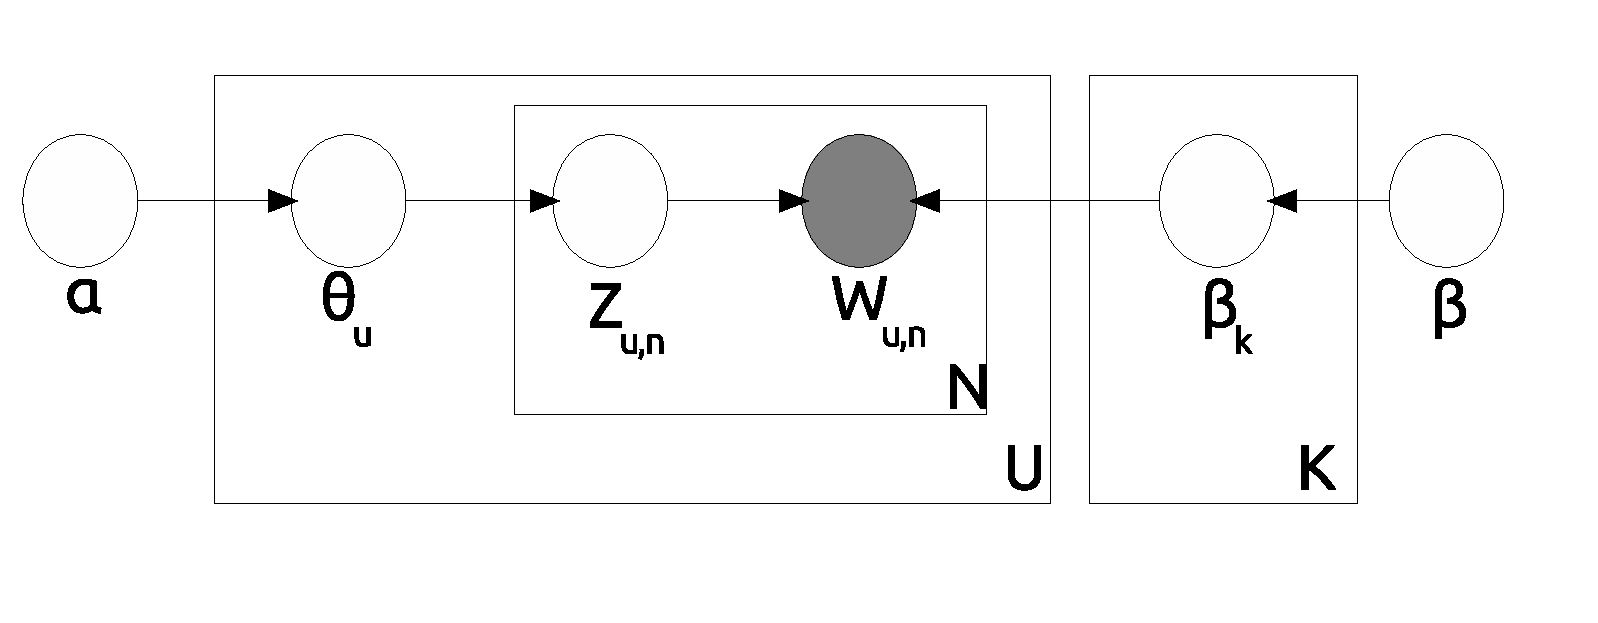
\includegraphics[width=3.0in,height=1.0in]{fig1.eps}
\caption{Plate illustration of the user-level LDA model.}
\label{fig1}
\end{figure}
To distill the topics that users are interested in, documents of LDA should naturally correspond to tweets content. 
As our goal is to understand the topics that each user is interested in rather than the topics each single tweet talks about, we aggregate the tweets published by each user into a single document, and replace documents of LDA with aggregated tweet documents. 
So a document stands for a s user in our model, and a user can be represented as a multinomial distribution over topics, which corresponds to the topic distribution of the user's subjectivity model.

Formally, given a set of users $ U $ and the number of topics $ K $, a user $u$ ($ u \in U $) could be represented by a multinomial distribution $ \theta_{u} $ over topics with a Dirichlet prior parameterized by $ \alpha $. 
A topic $ k $ ($ k \in K $) is represented by a multinomial distribution $ \beta_{k} $ with another Dirichlet prior parameterized by $ \eta $. 
The parameters $ \theta_{u} $ and each $ \beta_{k} $ can be estimated by Gibbs sampling or variational inference.
We use variational inference-based topic model package Gensim \cite{rehurek_lrec}.

\subsubsection{Opinion Analysis}
\label{sentiment}

Users often express opinions towards their topics of interest by publishing topic-related tweets. 
In order to explore the opinions of users, we need to understand sentiment embedded in each tweet.
Sentiment analysis mainly depends on machine learning or rule-based approaches. 
Machine learning approaches often need labelled data for the training process, which is often impossible for Twitter because of the large volume of tweets and its dynamic language characteristics. Therefore we adopt rule-based approaches, which could adapt to Twitter with good flexibility by changing its particular characteristics into rules \cite{Thelwall:2010SSS,Hu:2013www}.

The SentiStrength package has been built especially to cope with sentiment analysis in short informal text of social media \cite{Thelwall:2010SSS}. 
It combines lexicon-based approaches with sophisticated linguistic rules adapted to social media, which is suitable for analyzing sentiment of tweets in our research settings. 
SentiStrength assigns two values to each tweet standing for sentiment strengths: a positive (within $ [1,5] $) and a negative (within $ [-5,-1] $) sentiment measurement, both ranging from 1 to 5 on absolute integer scales, with 1 denoting neutral sentiment and 5 denoting highest sentiment strength. 
Sentiment assigned by SentiStrength is not a simple binary value but a fine-grained strength, which can catch fine opinion distributions in a user's subjectivity model. 
For the convenience calculation, we map the output of SentiStrength to a single-scaled sentiment valence space $ [0, 8] $ as follows: 
\begin{equation}
\label{opinionmap}
o= \left\{ 
\begin{array}{lll}
{p+3} &  \qquad if \; \vert p \vert > \vert n \vert \\
{n+5} &  \qquad if \; \vert n \vert > \vert p \vert \\
{4}  &   \qquad if \; \vert p \vert = \vert n \vert
\end{array}
\right.
\end{equation}
Where $ p $ denotes the positive setiment value and $ n $ denotes negative sentment value.
In the sentiment valence space $ [0, 8] $, value 4 indicates neutral sentiment, while values above 4 indicate positive sentiment and values below 4 indicate negative sentiment. With the sentiments of all tweets, we can aggregate opinions towards a topic as a sentiment distribution over sentiment valence space $ [0, 8] $.

\subsubsection{Concrete Subjectivity Model}
\label{concrete}

With statistical topic analysis and opinion analysis described above, we can concrete subjectivity model in a local network settings now. 
For user set $ U $ of a local network, we denote tweet set published by a user $ u $ as $ M_{u}=\left\lbrace m_{i} \vert i \in \left[ 1, \cdots, N \right]  \right\rbrace$. Each $ M_{u} $ is concatenated to a single document $ d_{u} $ to construct Local Topic Space $ T=\left\lbrace t_{i} \vert i=1, \cdots, K \right\rbrace $.
A topic model is built with parameter $ \theta $ representing the distribution of each user over topics in the Local Topic Space $ T $, and
parameter $ \beta $ represents the distribution of each topic over the vocabulary of all tweets. SentiStrength is applied to each tweet $ m $ in collection $ M_{u} $ and outputs sentiment strength $ s_{m} $ for tweet $ m $. 
We build the subjectivity model $ P(u) $ for user $ u $ as Algorithm~\ref{alg1}:

\begin{algorithm}[htb] 
\caption{ Establishment of subjectivity model .} 
\label{alg1}
\begin{algorithmic}[1] %这个1 表示每一行都显示数字
\REQUIRE ~~\\ %算法的输入参数:Input
The user set of a local network, $ U $;\\
The tweet set published by each user $ u $, $ M_{u} $;\\
\ENSURE ~~\\ %算法的输出:Output
The subjectivity model for each user $ u $, $ P(u) $;
\STATE Topic analysis with a user-level LDA as Section~\ref{topic}, getting a topic model $P(\theta,\beta|M_{u},U)$; 
\label{ alg1:topic }%对此行的标记,方便在文中引用算法的某个步骤
\FORALL {tweet $ m \in M_{u} $}
\label{alg1:sentiment}
\STATE Sentiment analysis as Section~\ref{sentiment}, outputting sentiment of $ m $, $ s_{m} $;
\ENDFOR
\FOR {user $ u \in U$}
\STATE the topic distribution is the corresponding component of parameter $ \theta $, $ \theta_{u} $; \\
\STATE the topics he tweets about are $ Z_{u}= \left\lbrace t \vert p\left( t \vert \theta_{u} \right)>0, t \in T \right\rbrace $; 
\ENDFOR
\FOR {tweet $ m \in M_{u} $}
\STATE topics of $ m $ can be identified by the topic model, $ Z_{m} =\left\lbrace t \vert p\left( t \vert \theta, \beta, Z_{u} \right)>0, t \in T \right\rbrace $; 
\ENDFOR
\FOR { each topic $ t \in Z_{u} $ }
\FOR { sentiment value $ s \in S $}
\STATE count the number of tweets which talk about topic $ t $ with sentiment value $ s $, $ N_{s}=\sum_{m \in M_{u}} I\left( s_{m} \right) ,  if  s_{m}=s \& t \in Z_{m} $; 
\ENDFOR
\STATE calculating opinion towards topic $ t $, $  O_{t} = \left\{ \frac{N_{s}}{\sum_{s \in S} N_{s}} \right\} $;
\ENDFOR
\STATE establishing subjectivity model of user $ u $, $ P\left( u \right)= \left\lbrace \left( t, p\left( t \vert \theta_{u} \right), \left\{ \frac{N_{s}}{\sum_{s \in S} N_{s}} \right\}  \right)  \vert t \in Z_{u}, s \in S  \right\rbrace   $;
\label{subuser}
\RETURN $P(u)$; %算法的返回值
\end{algorithmic}
\end{algorithm}
In the algorithm,  we assume the sentiment of tweet $ m $ is related to every topic it talks about in $ Z_{m} $ for simplicity.
Accordingly subjectivity model  $ P\left( m \right) $ for tweet $ m $ as:
\begin{equation}
\label{subtweet}
P\left( m \right)= \left\lbrace \left( t, p\left( t \vert \theta, \beta \right), d_{m,t}\left( s \right) \right)=1.0  \vert t \in Z_{m}, s \in S  \right\rbrace  
\end{equation}
Noting that, the opinion towards each topic is a distribution of $ 1.0 $ on a single sentiment value $ s $ of tweet $ m $.

\subsection{Retweeting Analysis With Subjectivity Model }
\label{formulation}

To understand the underlying reasons why a user retweet a message, we try to simulate the subjective decision-making procedure by investigating the relationship among the subjectivity models of a tweet, its author and followers. 
We assume that a user retweet a message because the user not only finds its topics interesting but also shares similar opinions towards these topics. In other words, if the subjectivity models of a tweet and a user are similar enough, the user will have a very high probability to retweet. 
We call this phenomenon as ``resonance'', and assume that the resonance between a tweet and users will elicit retweeting behavior.
With the subjectivity models built for users and tweets, we can define a similarity measurement to quantify the resonance among them.

Formally, for a tweet $ m $, the corresponding author $ a $, and a list of followers $ F= \left\lbrace f_{i} \right\rbrace  $, for each $ f_{i} \in F $, we can define a quadruple $ < f_{i}, a, m, r_{fam} >  $ as Section~\ref{statement}.
We firstly build subjectivity model  $ P\left( u \right)  $ for each user $ u \in F \bigcup p $ and $ P\left( m \right)  $ for tweet $ cm $, then define the similarity measurement as follows:
\begin{equation}
Sim\left( m,f_{i} \right) = similar\left( P\left( m \right), P\left( f_{i} \right) \right)
\end{equation}
according to Equation~\ref{subuser},\ref{subtweet}:
\begin{equation}
\label{tweetfollower}
\begin{split}
Sim\left( m,f_{i} \right) = \lambda \ast Dist\left( p\left(t \vert \theta, \beta, Z_{m} \right), p\left( t \vert \theta_{f_{i}}, Z_{f_{i}} \right) \right) \\
+\left(1-\lambda \right) \ast \left( \sum_{t \in T} Dist \left( O_{m,t}, O_{f_{i}, t} \right)  \right)
\end{split}
\end{equation}
where 
\begin{itemize}
\item $ \lambda $ is the coefficient used to control the proportions of topic similarity and opinion similarity in the holistic subjective similarity. We initiate it by setting $ \lambda =0.5 $, and adjust its value in the range of $ [0,1] $ to optimize the best performance of our model. 
\item $ Dist() $ is the similarity measurement between two distribution, we choose \emph{cosine distance } in our research among different measurements because of its effectiveness. 
\end{itemize}
We also assume that a user might retweet another user because of their subjective resonance. Accordingly we define similarity between author $ a $ and follower $ f_{i} $ as:
\begin{equation}
\label{pubfollower}
\begin{split}
Sim\left( a,f_{i} \right) = \lambda \ast Dist\left( p\left( t \vert \theta_{a}, Z_{a} \right), p\left( t \vert \theta_{f_{i}}, Z_{f_{i}} \right) \right) \\
+\left(1-\lambda \right) \ast \left( \sum_{t \in T} Dist \left( O_{a,t}, O{f_{i}, t} \right)  \right)
\end{split}
\end{equation}

\section{Experiment}
\label{experiment}

In this section, we investigate whether subjectivity model can help retweeting analysis on an Twitter dataset. 

\subsection{Dataset}

We adopt an off-the-shelf Twitter dataset of previous work \cite{Luo:2013RMF}, which was created with Twitter API\footnote{\url{https://dev.twitter.com/}}.
To form the dataset, 500 randomly selected English target tweets were monitored in the next few days to find followers who would retweet them. Also each target tweet was chosen as starting point to collect historical data of its author and followers. 
Overall, there are 45,531 followers and 6,277,736 tweets, and 5214 followers who have retweeted at least one target tweet during the monitored period. Summary statistics of the dataset are listed in Table~\ref{datasetstat}.
\begin{table}
\centering
\caption{Retweet Dataset Statistics}
\label{datasetstat}
\begin{tabular}{ll}
\hline
Tatget tweets  & 500 \\
\hline
Average number of followers per target tweet & 89 \\
Total retweeters & 5214 \\
Total non-retweeters & 40317  \\
\hline
\end{tabular}
\end{table}

The relations among a target tweet, its author and followers are illustrated in Figure~\ref{fig2}.
\begin{figure}[htb]
\centering
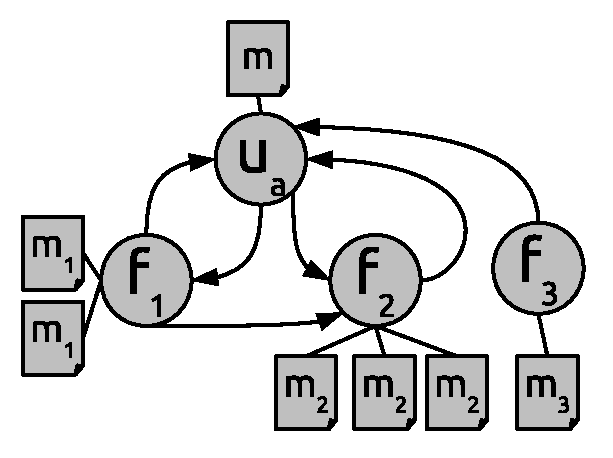
\includegraphics[width=1.5in,height=1.0in]{fig2.eps}
\caption{Relations among a target tweet, its author and followers.}
\label{fig2}
\end{figure}
There is a local network structure for each target tweet as figure shows, consisting of its author and followers.

\subsection{Impact Evaluation of Different Factors}
\label{influence}

In Section~\ref{formulation}, we model retweeting probability with subjectivity model in the form of similarity measurements~\ref{tweetfollower},\ref{pubfollower}.
By setting different value to $ \lambda $, the measurements can be transformed into different versions to model different factors that might influence user's retweeting behavior, which are:
\begin{itemize}
\item \textbf{TTF}: \textbf{T}opic similarity between \textbf{T}weet and \textbf{F}ollower ($\lambda =1$ in measurement~\ref{tweetfollower}). 
\item \textbf{OTF}: \textbf{O}pinion similarity between \textbf{T}weet and \textbf{F}ollower ($ \lambda =0 $ in measurement~\ref{tweetfollower}). 
\item \textbf{STF}: \textbf{S}ubjective similarity between \textbf{T}weet and \textbf{F}ollower ($ \lambda \in ( 0,1 ) $ in measurement~\ref{tweetfollower}).  
\item \textbf{TAF}: \textbf{T}opic similarity between \textbf{P}ublisher and \textbf{F}ollower ($ \lambda =1 $ in measurement~\ref{pubfollower}).  
\item \textbf{OAF}: \textbf{O}pinion similarity between \textbf{P}ublisher and \textbf{F}ollower ($ \lambda =0 $ in measurement~\ref{pubfollower}).
\item \textbf{SAF}: \textbf{S}ubjective similarity between \textbf{P}ublisher and \textbf{F}ollower ($ \lambda \in ( 0,1 ) $ in measurement~\ref{pubfollower}). 
\end{itemize}
The six similarity measurements could be grouped into two aspects. 
One is consisted of TTF, OTF and STF, which is direct and explicit by modelling the tweet and its followers;
the other is consisted of TAF, OAF and SAF, which is indirect and implicit by modelling the author and follower.
The two aspects reflect properly the local information diffusion structure of Twitter at micro-level as illustrated in Figure~\ref{fig2}.

To evaluate the impact of different factors on retweeting behavior, we compare six average similarity scores between 5214 retweeters and 5214 randomly selected non-retweeters. The values of $ \lambda $ for STF and SAF are tuned to produce the largest value difference between retweeters and non-retweeters, which are $ \lambda =0.5 $ on our dataset. Figure~\ref{fig3} shows the result.
\begin{figure}[htb]
\centering
\includegraphics[width=3.0in,height=2.0in]{fig3.eps}
\caption{Impact of different factors on retweeting behavior.}
\label{fig3}
\end{figure}
As the figure illustrated, the similarities scores of retweeters are obviously higher than non-retweeters for all six factors. Specifically: 
\begin{itemize}
\item TTF score shows that a tweet is more likely to be retweeted by followers who find topics it talks about interesting to them, which is consistent with other studies\cite{conf/icwsm/MacskassyM11};
\item OTF score shows that opinions in a tweet is an important indicator to be retweeted by by followers who hold similar opinions, although other studies\cite{conf/icwsm/PfitznerGS12,2011:NaveedGKC} have shown that sentiment in tweet has impact on retweeting behavior, they haven't consider the opinions of followers and opinion similarity betweet tweet and followers;
\item STF score shows the subjective similarity is the most distinguishable feature among the six factors with the largest value difference, which proves the importance of subjectivity model;
\item TAF score gives another perspective for retweeting analysis from the topic similarity between author and followers, indicating that followers are more likely to retweet author with similar interests , which verifies the homophily principle of following relation;
\item OAF score indicates that similar opinions also influence followers' decision of retweeting another user, which proves opinion homophily of following relation.
\item SAF score is interesting in that it implies that subjective similarity between author and followers might cause retweeting, and we call this phenomenon ``tight homophily'' of following relation because it requires both topic homophily and opinion homophily.
\end{itemize} 

\subsection{Performance of Retweeting Prediction}
\label{performance}

The main purpose of retweeting analysis is to help users find interesting information from the overwhelming information streams. 
Retweeting is an important signal of interestingness because users are prone to broadcast their favorite messages to their followers. 
Thus, the performance of retweeting prediction is a suitable evaluation for the utility of subjectivity model in retweeting analysis problem. 
In our experiment, we evaluate the subjectivity model in supervised machine learning framework.

As Section~\ref{statement} introduced, the retweeting analysis problem could be formulated as a quadruple $< f, a, c, r_{fam} > $. 
For retweeting prediction, we need to estimate the label $ r_{fam} $ when $ m, a, and  f $ are known. 
There are 5,214 retweeters in our dataset who retweet at least one target tweet, so we extract 5214 quadruples as positive instances with their label $ r_{fam}=1 $. 
For the other 40,317 non-retweeters, we also extract quadruples as negative instances with label $ r_{fam}=0 $. 
To avoid unbalance bias of training data, we randomly sample 5,214 negative instances into the test dataset. 

\subsubsection{Comparison With Other User Models}
\label{comparison}

Firstly the comparison between our model with other UGC-based user models (TF-IDF model \cite{Luo:2013RMF}, entity-based model and hashtag-based model \cite{Abel:2011AUM}) in retweeting prediction is investigated. 
As defined in Section~\ref{influence}, the six similarities derived from our model are used for comparison, because they model different factors that influence retweeting baehavior. 
For the comparing models, cosine similarities are calculated between tweets and followers.
We use the logistic regression classifier of Scikit-learn machine learning package \cite{scikit-learn}, with 5-fold cross-validation on our balance dataset. Accuracy is our evaluation metric.
Performances of our model and all other models are shown in Figure~\ref{fig4}.
\begin{figure}[htb]
\centering
\includegraphics[width=3.5in,height=2.2in]{fig4.eps}
\caption{Comparison of different models.}
\label{fig4}
\end{figure}
Figure~\ref{fig4} also shows that the impact of topic number of LDA on the predicting accuracy, our model arrives its peak when the number is set to 60, so we fix the topic number as 60 in all our experiment. 

As Figure~\ref{fig4} illustrates, the best accuracy of 68.67\% is achieved by the STF (Subjective similarity between tweet and followers). 
The accuracies of TF-IDF model and entity-based model are 63.45\% and 62.12\%, which are very close to TTF (Topic similarity between Tweet and Followers, 63.88\%) and OAF (Opinion similarity between Publisher and Followers, 62.96\%). 
While for hashtag-based model, its accuracy is 50.76\% , which is only a little better than random selection (50\%) but not significant. The reason might lie in a very low usage of hashtag in our data. 
The accuracies of the other three model are OTF (Opinion similarity between Tweet and Followers, 64.80\%), TAF (Topic similarity between Publisher and Followers, 62.58\%) and SAF (Subjective similarity between Publisher and Followers, 66.95\%) model. 
The results show that subjectivity model can better help understanding retweeting behavior than the other user models.

\subsubsection{Comparison with Other Factors}
\label{classifiction}

In this section, we feed the six similarities of our model as features into a retweeting classification framework to verify the effectiveness of subjectivity model. 
We compare the performance of our model with method of Luo \emph{et al.}~\cite{Luo:2013RMF} which uses four feature families: Retweet History (follower who retweeted a user before is likely to retweet the user again), Follower Status (for a follower, the number of tweets, followers, friends, being listed and whether he is verified), Follower Active Time (the time users interact with others) and Follower Interests (common interests between tweet and followers, TF-IDF model).

We use LinearSVM of Scikit-learn package to build a retweeting prediction framework, leveraging two different features sets. One includes the six features derived from subjectivity model (marked as ``SM6''). The other is the feature set from Luo \emph{et al.}~\cite{Luo:2013RMF} (marked as ``LUO''). We use the same dataset as Section~\ref{comparison} with 5-fold cross-validation, and accuracy as evaluation metric. 
In addition, we set a baseline (marked as ``RB''), for which followers who have retweeted the author's previous tweets are predicted as retweeters of current tweet. 
The result is listed in Table~\ref{table2}. 
\begin{table}
\centering
\caption{Prediction Accuracy of Different Models. Significant improvement over baseline with star($ \ast $) and LUO' model with dagger($ \ddagger $) (p$ < $0.05).}
\label{table2}
\begin{tabular}{ll}
\hline
Feature Set & Accuracy(\%) \\
\hline
RB & 60.85  \\
LUO & 68.76 $ \ast  $\\
SM6 & 69.12  $ \ast $ \\
LUO($ \ominus $)+TTF & 69.20  $ \ast $ \\
LUO($ \ominus $)+TAF & 71.04  $ \ast \quad \ddagger $ \\
LUO($ \ominus $)+OTF & 71.88  $ \ast \quad \ddagger $ \\
LUO($ \ominus $)+OAF & 70.27  $ \ast $ \\
LUO($ \ominus $)+STF & 72.86  $ \ast \quad \ddagger $ \\
LUO($ \ominus $)+SAF & 72.05  $ \ast \quad \ddagger $ \\
LUO($ \ominus $)+All & 72.93  $ \ast \quad \ddagger $ \\
\hline
\end{tabular}
\end{table}
The accuracy of baseline is 60.85\%, and two prediction models (LUO and our SM6) both outperform the baseline significantly. 
But the prediction model based on our feature set shows no significant improvement over LUO feature set. 
The reason might be that our model only tries to reflect the retweeting motivation of users based on content, whereas other important factors associated with retweeting behavior are not considered, such as network topology and tweeting habit of the user, etc. 

Since it is proved that subjectivity model outperforms TF-IDF model in Section~\ref{comparison}, which is used in LUO feature set, we propose that retweeting prediction performance could be improved by using features derived from subjectivity model. 
As denoted by ``LUO($ \ominus $)+'' in the table, the Follower Interests features of LUO are replaced with our six features one by one. 
The accuracies are all improved. It shows that our model is of great importance for retweeting prediction. 
Noticing that, the most significant improvement (LUO($ \ominus $)+STF, 72.86\% versus 68.76\%) is the subjective similarity feature between tweet and followers, which verifies our assumption that subjective resonance between tweet and followers can be considered as the underlying reason that elicits retweeting behavior. 
Besides, the improvement by adding subjective similarity features between aauthor and followers (LUO($ \ominus $)+SAF, 72.05\% versus 68.76\%) is also obvious in that the resonance between author and follower indicates the tight homophily between them. 
Finally, the last row of table is the complete combination of two sets of features (LUO($ \ominus $)+All) by adding all six features into LUO feature set. 
The performance shows no significant improvement over adding STF feature only, in that subjectivity model combines both topic and opinion information, and STF is a integral feature to model both topic similarity and opinion similarity between tweet and followers, so it is redundant to add other separate parts. 

\subsection{Case Study}
\label{example}
In this section we give an vivid example to illustrate the subjectivity model and its ability in explaining the retweet behavior. 
The subjectivity models for one of the 500 target tweets, its author, and two followers (one retweeter, the other non-retweeter) are shown as Figure~\ref{fig5}. 
The right part of each sub-figure illustrates topic distribution and the left part illustrates opinions towards each topic. 
It is the $ 14^{th} $ topic that the tweet talks about in the local topic space. 
\begin{figure*}[htb]
\centering
\includegraphics[width=5.5in,height=3.2in]{fig5.eps}
\caption{Subjectivity models of tweet, author and followers.}
\label{fig5}
\end{figure*}
Figure~\ref{fig6} shows top words of the $ 14^{th} $ topic, the tweets of author and two followers in a word cloud\footnote{We use TagCrowd (\url{http://tagcrowd.com/}) to produce word cloud.}.
\begin{figure}[htb]
\centering
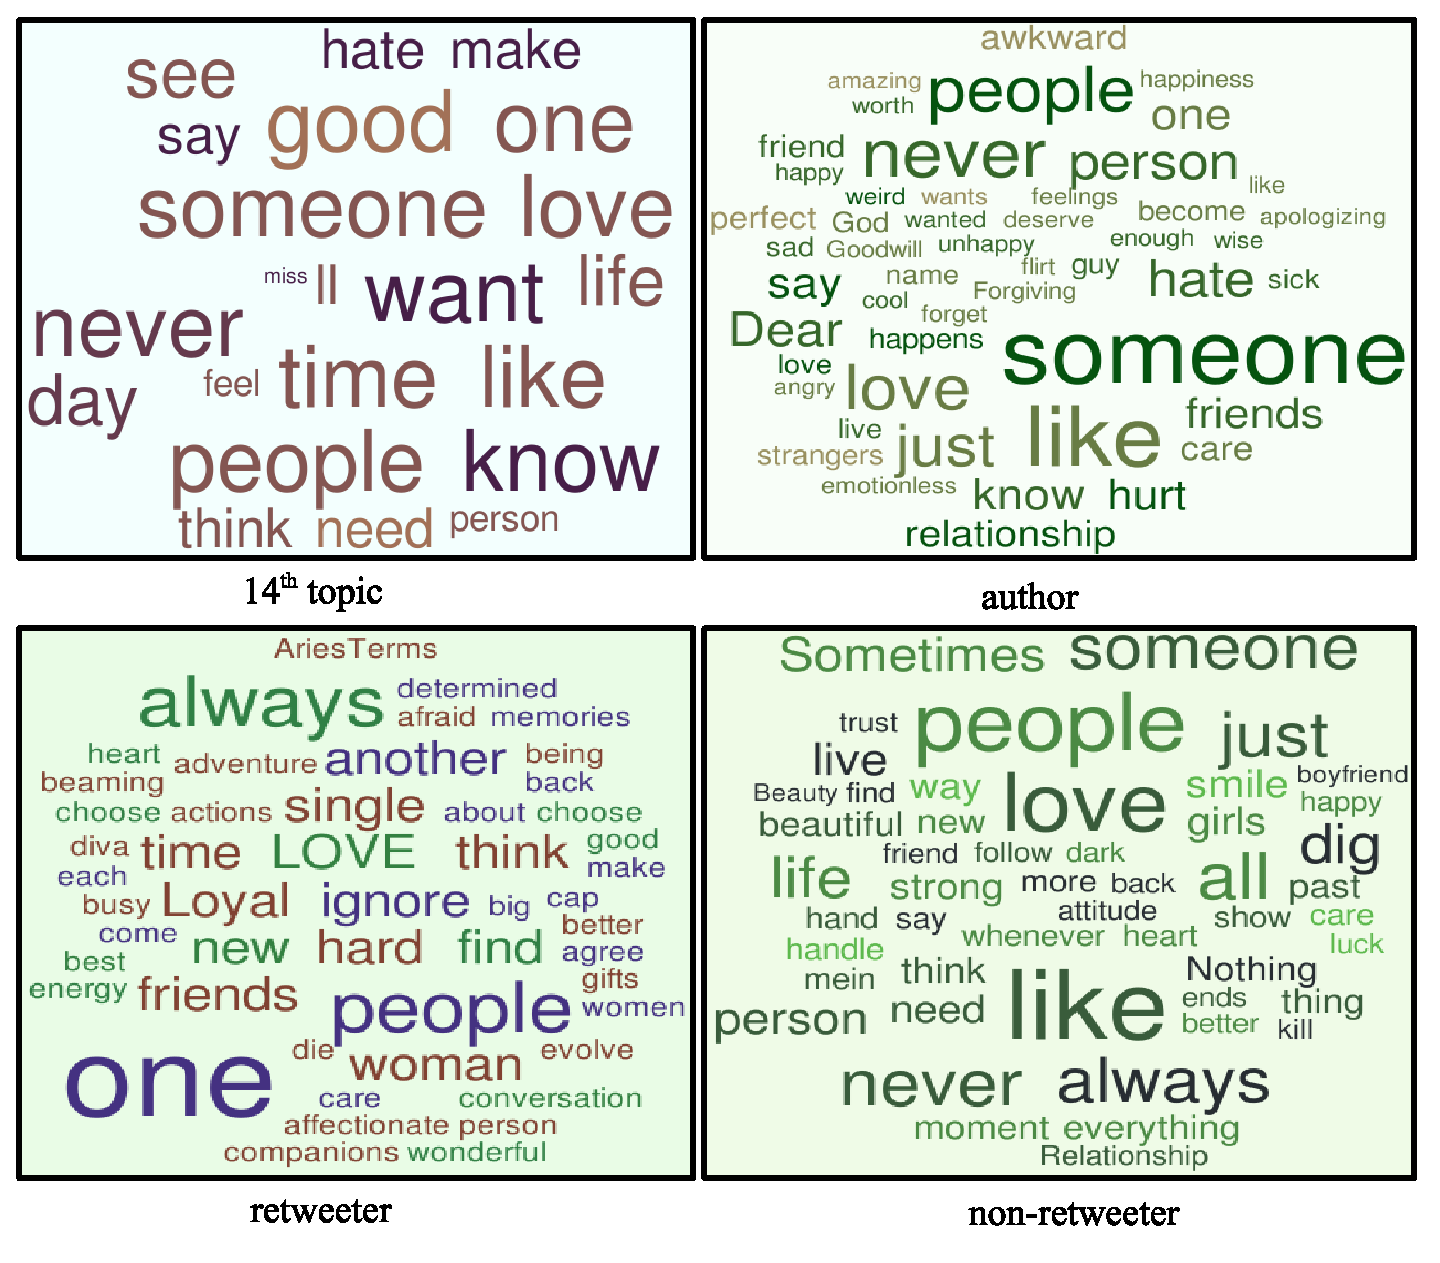
\includegraphics[width=3.2in,height=2.0in]{fig6.eps}
\caption{Word cloud of $ 14^{th} $ topic, author and followers.}
\label{fig6}
\end{figure}
Content of the tweet is:\\
\textit{Tweet: ``Sometimes the right person for you was there all along. You just didn’t see it because the wrong one was blocking the sight''} \\
The topic of this tweet is about ``love between people'' and the opinion is neutral, which is in accordance with the $ 14^{th} $ topic word cloud in Figure~\ref{fig6} and subjectivity model of tweet in Firgure~\ref{fig5}.
The author concentrates on the $ 14^{th} $ topic with 208 tweets, and his opinions are mainly neutral (as Figure~\ref{fig5},~\ref{fig6} demonstrate). 
As for two followers, the retweeter has published 250 tweets about two topics (the $ 14^{th} $ and $ 52^{nd} $ topic) uniformly and his opinions towards the two topics are mainly neutral. 
While the other one, the non-retweeter has also talked about two topics ($ 14^{th} $ and $ 56^{th} $ topic) with 188 tweets, but he is mainly interested in the $ 14^{th} $ topic and his opinion is positive.
Although two followers have same interest (the $ 14^{th} $ topic), their different opinions elicit their different decision, which verifies subjectivity model can help better understanding the retweeting behavior not only from topics but also opinions. 

\section{Conclusion}
In this paper, we propose a subjectivity model to analyze user retweeting behavior on Twitter. We assume that retweeting should be elicited by the subjective resonance between the tweet and its followers. 
We define the subjectivity model formally as the combination of topics and opinions, and we put forward an algorithm to establish the subjectivity model leveraging statistical topic model and sentiment analysis techniques. 
We demonstrate the effectiveness of our model for retweeting analysis problem and show that subjectivity model is able to reach better understanding of retweeting behavior. 

Our future work mainly lie in two directions. 
Firstly, the subjectivity model is established through simple combination of topics and opinions. It is an interesting direction to establish it under the framework of generative topic-sentiment model, which has been applied in reviews and citation network. 
Secondly, we will apply subjectivity model to other social media analysis task such as connection prediction and friend recommendation. 


%\begin{acknowledgements}
%If you'd like to thank anyone, place your comments here
%and remove the percent signs.
%\end{acknowledgements}

% BibTeX users please use one of
%\bibliographystyle{spbasic}      % basic style, author-year citations
%\bibliographystyle{spmpsci}      % mathematics and physical sciences
%\bibliographystyle{spphys}       % APS-like style for physics
%\bibliography{}   % name your BibTeX data base

% Non-BibTeX users please use


\bibliographystyle{spmpsci}
\bibliography{resonate_tweet}
\end{document}
% end of file template.tex

